\section{Experiment}

We tested our algorithm to detect humans. Table \ref{table:1} shows the components used as follows:

\begin{table}[h]
\begin{center}
\begin{tabular}{ | m{3.5cm} | m{3.5cm}| } 
\hline
\textbf{Classification Model} & \textbf{Detection Model} \\ 
\hline
Operating System & Raspbian OS \\
\hline
CPU & Braodcom 1.5 GHz quad-core A72 64-bit \\
\hline
GPU & Broadcom VideoCore VI  \\
\hline
Memory & 8GB \\
\hline
Tensorflow & 1.15 \\
\hline
Camera Sensor & Raspberry Pi Camera Board v2 8MP \\
\hline
\end{tabular}
\caption{Experimental Environment}
\label{table:1}
\end{center}
\end{table}

There are many techniques used. However, the mainly used activations are sigmoid, tanh, relu and leaky relu \cite{Chauhan}. These techniques, along with COCO, allowed us to train our algorithm to for the detection of humans, regardless of of the type of clothing worn. As demonstrated in figure \ref{fig:fig1_e}, the algorithm detects a person. The training set was trained using pre-trained models of each classification model. The accuracy of the algorithm depends on the type of camera used. To reduce high variance, regularization techniques
and data augmentation techniques can be implemented. Another technique to reduce overfitiing is to train the data on large datasets. We used a Raspberry Pi Camera Board v2 8MP to perform our experiment. We believe that using a higher quality camera will produce better results. The algorithm is able to detect a person, even if there is movement. As demonstrated in figure \ref{fig:fig2_e}, the algorithm is able to detect the person, regardless of the person's previous position. This is important since the algorithm must be able to detect fast moving objects. Our setup was limited by the hardware we used, nevertheless we predict the algorithm can be trained to be far more efficient. For experimental purposes, we decided that a simple setup was satisfactory enough for our needs.

The accuracy of the sensor also showed is weakness as the light source diminished. This means, the darker the scene, the lesser the accuracy of the algorithm becomes. However, our experiment shows that the algorithm can detect individual that steal packages, which mostly happens during the day, in broad daylight. Most of the limitations we faced were centered around hardware deficiencies. Conversely, conducting the experiment was done in a more ideal environment. This means lighting conditions were ideal, distance from the sensor was 24cm and the test subject was relatively in the line of sight of the sensor, meaning the test object was not at a difficult angle for the sensor to detect. Additionally, we were not able to test a multitude of test subjects, although we are confident that the algorithm would be able to detect them. Our goal was to produce an algorithm that detects a small group of people, since home invasions, burglaries and package snatching typically involves a small group of individuals.

\begin{figure}
    \centering
    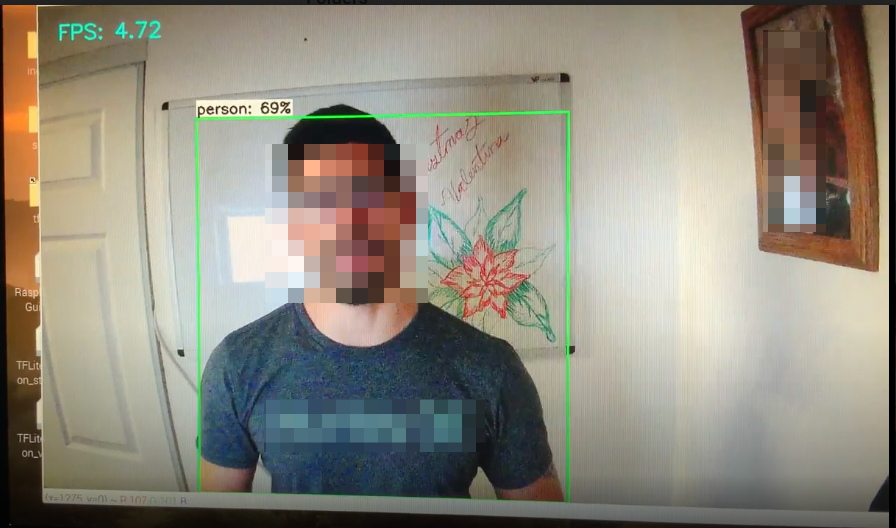
\includegraphics[width=6cm]{Security Object Detection, Surveillance/Latex/figures/fig1_e.png}
    \caption{Computer vision detecting a person}
    \label{fig:fig1_e}
\end{figure}

\begin{figure}
    \centering
    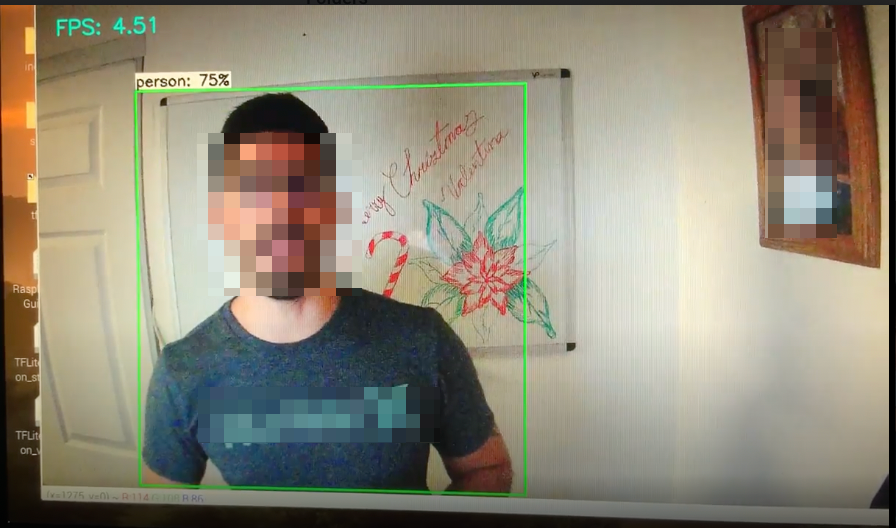
\includegraphics[width=6cm]{Security Object Detection, Surveillance/Latex/figures/fig2_e.png}
    \caption{Even if the person moves, the algorithm is able to detect the change}
    \label{fig:fig2_e}
\end{figure}
